\section{Описание работы программного модуля: }
\begin{itemize}
    \item На экране отображается дорога в три полосы движения.  Внизу экрана находится автомобиль.;
    \item При открытии страницы из-за верхней границы экрана вниз по одному начинают двигаться булыжники по одной из полос (имитируя движение автомобиля).;
    \item Пользователь управляет автомобилем, нажимая клавиши “A” и “D”. Автомобиль  может  находиться в трех положениях: на первой полосе, второй или третьей.; 
    \item Если автомобиль и булыжник пересекутся своими границами, вместо автомобиля и камня отобразится взрыв.;
\end{itemize}
    \begin{figure}[H]
	\begin{center}
		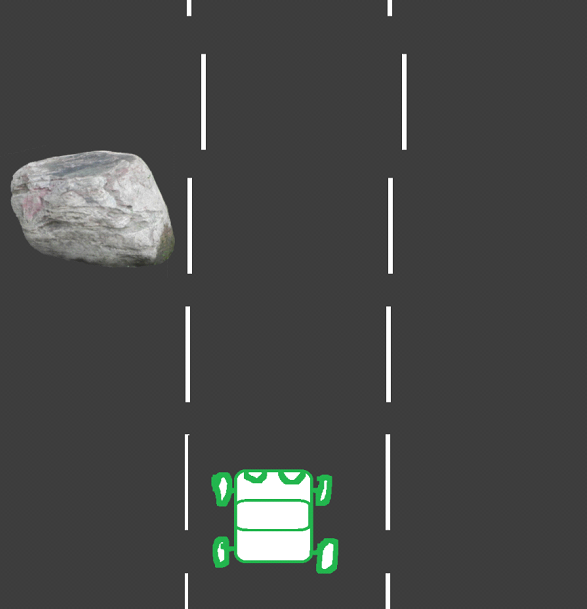
\includegraphics[scale=1]{fig/image.png}
		\caption{Внешний вид интерфейса}
		\label{pic:fig/image.png} % название для ссылок внутри кода
	\end{center}
    \end{figure}
     
    Цель Работы: провести тестирование программного модуля с использованием событий клавиатуры, написать формулу кинетической энергии до столкновения камня с машиной.

    При тестировании обращаться к \cite{ref-book}\
    
    Описание особенностей тестируемого программного модуля: В данном программном модуле особое внимание уделено использованию событий клавиатуры. 
    
    Выполненные виды тестирования: 
\begin{itemize}
    \item Тестирование функционала: ;
    \begin{itemize}
    \item Вместо камня не показывался взрыв.;
    \item После щелчка выполнялось сразу несколько условий, поэтому перемещение автомобиля работало некорректно. Был добавлен return в конце условий.;
    \item Автомобиль перемещается и после взрыва. Добавлена проверка на взрыв автомобиля.; 
\end{itemize}
\begin{code}
	\inputminted[breaklines=true, xleftmargin=1em, linenos, frame=single, framesep=10pt, fontsize=\footnotesize, firstline=1]{haskell}{listings/code.js}
	% \caption{Script.bash – bash в массы!}
    \end{code}
    \item Оценка интерфейса удобства использования веб-приложения:;

    Интерфейс приятен для восприятия

    \item Оценка кроссбраузерности:
    
Результат оценки представлен в таблице ~\ref{tab_1}
    
\end{itemize}

\begin{table}[H]
	\caption{Оценка кроссбраузерности:}
	\begin{center}
		\begin{tabular*}{\textwidth}{@{\extracolsep{\fill} } lccc}
			\toprule
			Yandex & InternetExplorer & Chrome & FireFox \\
			\midrule
			Работает корректно       & Работает корректно    & Работает корректно & Работает корректно    \\
			\bottomrule
		\end{tabular*}
		\label{tab_1}
	\end{center}
\end{table}

    \item Формула кинетической энергии  ~\ref{eq:eq1}

    
    \begin{equation}
        \centering
        \label{eq:eq1}
        K=\frac{m_{1}v_{1}^{2}}{2} + \frac{m_{2}v_{2}^{2}}{2}
    \end{equation}
    
\newpage
\section{Заключение}
Вывод: в ходе выполнения лабораторной работы было проведено тестирование программного модуля с использованием событий клавиатуры.
